\documentclass[12pt]{article}
\usepackage[utf8]{inputenc}
\usepackage[T1]{fontenc}
\usepackage{amsmath}
\usepackage{amssymb}
\usepackage{geometry}
\geometry{a4paper, margin=1in}
\usepackage{booktabs}
\usepackage{enumitem}
\usepackage{listings} % For code sections with line numbers
\lstset{
    basicstyle=\ttfamily\small,
    numbers=left,
    numberstyle=\tiny,
    stepnumber=1,
    numbersep=5pt,
    showspaces=false,
    showstringspaces=false,
    frame=single,
    breaklines=true,
    breakatwhitespace=true,
    captionpos=b,
    backgroundcolor=\color{lightgray!20} % Light gray fill for code blocks
}
\usepackage{xcolor} % For background color
\usepackage{tikz} % For network diagram
\usetikzlibrary{arrows.meta, positioning}

% Mathematical and table packages
\usepackage{amsfonts}
\usepackage{stackrel}

% Font configuration (last in preamble)
\usepackage{DejaVuSans} % Default font for Latin and compatible scripts

% Setting the title, author, and date
\title{Examination Paper: Boolean Network Pattern Analysis for AI and Data Science Candidates}
\author{}
\date{June 19, 2025}

\begin{document}

\maketitle

\begin{abstract}
This examination paper presents two challenging problems related to pattern analysis in Boolean networks, targeting prospective data scientists, AI experts, and software developers. The purpose is to evaluate candidates' abilities to solve problems across diverse technical domains, adapt to unfamiliar technologies, leverage AI tools independently, document complex ideas, explore novel tools, and utilise unknown code as black boxes. Candidates must develop solutions, document them in LaTeX, and submit them via a GitHub repository, demonstrating a comprehensive skill set suitable for advanced roles in artificial intelligence and machine learning.
\end{abstract}

\section{Introduction}
The objective of this examination is to identify and recruit three exceptional professionals in the fields of artificial intelligence (AI), machine learning (ML), and software development. The selection process seeks individuals with a proven capacity to solve problems across a wide range of technical challenges, not merely limited to discerning patterns but extending to addressing varied issues in technology. Key qualities under evaluation include the ability to locate and utilise appropriate technologies to tackle unexpected problems, the skill to harness AI tools without prior guidance, the competence to communicate intricate concepts effectively in written and verbal forms, the willingness to engage with novel, infrequently used technologies, and the capability to adapt and utilise unknown code as black boxes.

Additional desirable attributes encompass analytical thinking, attention to detail, and the ability to work independently under ambiguous conditions. Candidates may employ any tools, including large language models (LLMs), to leverage the latest advances in AI. However, the evaluation prioritises individuals who avoid 'vibe-code'—blind reliance on code or material generated by AI—and instead demonstrate the capacity to critically assess, adapt, and create imaginative, disruptive solutions. This examination challenges candidates to exhibit these skills through two distinct problems, seeking non-iterative, elegant solutions reminiscent of \( F = ma \) or \( E = mc^2 \), rather than exhaustive computations. Success in this assessment will indicate a candidate's readiness to contribute innovatively to cutting-edge projects in AI and data science, with shorter completion times enhancing their prospects for selection.

\section{Explanation of the Problem}
\subsection{Background on Boolean Networks}
Boolean networks model complex systems where nodes represent entities, and directed edges (arrows) define interactions. A network with \( n \) nodes uses an \( n \times n \) adjacency matrix \( C \), where \( C_{i,j} = 1 \) indicates that node \( i \) receives input from node \( j \), and \( C_{i,j} = 0 \) otherwise. The dynamics list \( D \) specifies each node’s Boolean function (e.g., AND, OR), defining how a node processes inputs. In a real-run scenario, a node \( k \) aggregates inputs from nodes \( i \) where \( C_{k,i} = 1 \), computes its output based on \( D[k] \) (e.g., AND requires all inputs to be 1), and delivers this result to nodes \( j \) where \( C_{j,k} = 1 \).

Consider a 4-node network arranged in a ring with additional connections, as shown in Figure~\ref{fig:network_diagram}, where nodes 1 and 3 have multiple inputs. The adjacency matrix and dynamics list can be defined in Mathematica as follows:
\begin{lstlisting}[caption={Mathematica Definition of 4-Node Network}]
n = 4;
cm = {{0, 1, 0, 1}, 
      {1, 0, 1, 0}, 
      {0, 1, 0, 1}, 
      {1, 0, 1, 0}};
dyn = {"AND", "OR", "AND", "OR"};
\end{lstlisting}
\begin{figure}[h]
    \centering
    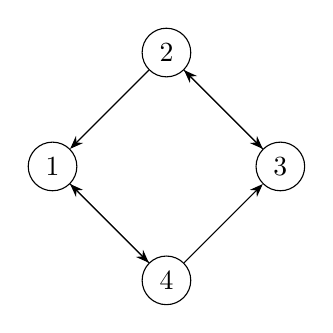
\begin{tikzpicture}[node distance=2cm, every node/.style={circle, draw}]
        \node (1) at (0,0) {1};
        \node (2) [above right=1cm and 1cm of 1] {2};
        \node (3) [below right=1cm and 1cm of 2] {3};
        \node (4) [below left=1cm and 1cm of 3] {4};
        \draw[-{Stealth}] (2) -- (1);
        \draw[-{Stealth}] (3) -- (2);
        \draw[-{Stealth}] (4) -- (3);
        \draw[-{Stealth}] (1) -- (4);
        \draw[-{Stealth}] (4) -- (1); % Additional connection
        \draw[-{Stealth}] (2) -- (3); % Additional connection
    \end{tikzpicture}
    \caption{Diagram of a 4-node Boolean network arranged in a ring with additional connections.}
    \label{fig:network_diagram}
\end{figure}

The input repertoire consists of all \( 2^n \) binary vectors, generated exhaustively and ordered. For \( n = 4 \), starting from index 1 (1-based) and reading left to right (most significant bit first, as reversed by `allPosibleInputsReverse`), the list is:
\begin{center}
\begin{tabular}{c|c}
\textbf{Index} & \textbf{Binary Vector} \\
\hline
1 & (0,0,0,0) \\
2 & (0,0,0,1) \\
3 & (0,0,1,0) \\
4 & (0,0,1,1) \\
5 & (0,1,0,0) \\
6 & (0,1,0,1) \\
7 & (0,1,1,0) \\
8 & (0,1,1,1) \\
9 & (1,0,0,0) \\
10 & (1,0,0,1) \\
11 & (1,0,1,0) \\
12 & (1,0,1,1) \\
13 & (1,1,0,0) \\
14 & (1,1,0,1) \\
15 & (1,1,1,0) \\
16 & (1,1,1,1) \\
\end{tabular}
\end{center}

An AND gate at node 1, with inputs from nodes 2 and 4 (\( C_{1,2} = 1 \), \( C_{1,4} = 1 \)), outputs 1 only if both \( v_2 = 1 \) and \( v_4 = 1 \). The output repertoire, computed step-by-step, is shown as a truth table:
\begin{center}
\begin{tabular}{c|c|c|c|c|c}
\textbf{Index} & \textbf{Input (v)} & \textbf{Node 1 (AND)} & \textbf{Node 2 (OR)} & \textbf{Node 3 (AND)} & \textbf{Node 4 (OR)} \\
\hline
1 & (0,0,0,0) & 0 & 0 & 0 & 0 \\
2 & (0,0,0,1) & 0 & 0 & 0 & 1 \\
3 & (0,0,1,0) & 0 & 1 & 0 & 0 \\
4 & (0,0,1,1) & 0 & 1 & 0 & 1 \\
5 & (0,1,0,0) & 0 & 1 & 0 & 0 \\
6 & (0,1,0,1) & 0 & 1 & 0 & 1 \\
7 & (0,1,1,0) & 0 & 1 & 0 & 1 \\
8 & (0,1,1,1) & 0 & 1 & 0 & 1 \\
9 & (1,0,0,0) & 0 & 1 & 0 & 1 \\
10 & (1,0,0,1) & 0 & 1 & 0 & 1 \\
11 & (1,0,1,0) & 0 & 1 & 0 & 1 \\
12 & (1,0,1,1) & 0 & 1 & 0 & 1 \\
13 & (1,1,0,0) & 0 & 1 & 0 & 1 \\
14 & (1,1,0,1) & 1 & 1 & 0 & 1 \\
15 & (1,1,1,0) & 0 & 1 & 0 & 1 \\
16 & (1,1,1,1) & 1 & 1 & 1 & 1 \\
\end{tabular}
\end{center}
This table shows how each node’s output evolves based on its function and inputs.

Applicants are provided with the following optimised Mathematica functions to compute repertoires, which they may use as black boxes:
\begin{lstlisting}[caption={Optimised Mathematica Functions for Repertoire Computation}]
myOr[list_] := Boole[MemberQ[list, 1]];
myNand[list_] := Boole[! FreeQ[list, 0]];
myAnd[list_] := Boole[FreeQ[list, 0] && Length[list] > 0];
myXor[list_] := Mod[Total[list], 2];
allPosibleInputsReverse[noNodes_] := Reverse /@ IntegerDigits[Range[0, 2^noNodes - 1], 2, noNodes];
getIndexesOfNodesInputs[node_, cm_] := Sort[Flatten[Position[cm[[node]], 1]]];
getListInputsByIndex[input_, indexes_] := Part[input, indexes];
runDynamic[cm_, dynamic_] := Module[{noNodes, inputs, repertoireResultsNet},
    noNodes = Length[dynamic];
    inputs = allPosibleInputsReverse[noNodes];
    repertoireResultsNet = MapIndexed[
        Module[{indexes = getIndexesOfNodesInputs[#2[[1]] - 1, cm], inputsToNode = getListInputsByIndex[#1, indexes], nodeOp = dynamic[[#2[[1]]]]},
            Which[
                nodeOp === "AND", myAnd[inputsToNode],
                nodeOp === "OR", myOr[inputsToNode],
                nodeOp === "XOR", myXor[inputsToNode],
                nodeOp === "NAND", myNand[inputsToNode],
                True, 0
            ]
        ] &,
        inputs,
        {2}
    ];
    <|"RepertoireInputs" -> inputs, "RepertoireOutputs" -> repertoireResultsNet|>
];
filterByCondition[inRep_, outRep_, indexElement_, expectedOut_] := Module[{indexes, ins, outs},
    indexes = Flatten[Position[outRep[[All, indexElement]], expectedOut]];
    ins = inRep[[indexes]];
    outs = outRep[[indexes]];
    <|"indexes" -> indexes, "ins" -> ins, "outs" -> outs|>
];
\end{lstlisting}
The ability to effectively utilise such unknown code as black boxes constitutes an additional skill under evaluation.

\subsection{Problem 1: Pattern Analysis in Input Repertoires}
As described in the background section, consider a Boolean network with \( n \) nodes, where connectivity is defined by an \( n \times n \) adjacency matrix \( C \), and the dynamics list \( D \) specifies each node’s Boolean function. The input repertoire comprises all \( 2^n \) possible binary vectors \( \{b_1, b_2, \dots, b_n\} \), where \( b_i \in \{0, 1\} \), indexed from 1 to \( 2^n \). Each index \( j \) corresponds to the binary representation of \( j-1 \), with \( b_1 \) as the most significant bit (leftmost, as reversed by `allPosibleInputsReverse`).

Given a subset of nodes \( \{k_1, k_2, \dots, k_m\} \subseteq \{1, 2, \dots, n\} \) and a desired pattern \( \{p_1, p_2, \dots, p_m\} \), where \( p_i \in \{0, 1\} \), determine all indices \( j \in \{1, 2, \dots, 2^n\} \) such that the \( k_i \)-th bit of the binary vector at index \( j \) equals \( p_i \) for all \( i = 1, 2, \dots, m \).

\subsection{Problem 2: Output Pattern of AND Gates}
As outlined in the background section, consider a Boolean network with \( n \) nodes, represented by an \( n \times n \) adjacency matrix \( C \), where the dynamics list \( D \) assigns each node a Boolean function, with node \( k \) using AND. The input repertoire consists of \( 2^n \) binary vectors \( v = (v_1, v_2, \dots, v_n) \), where \( v_i \in \{0, 1\} \), indexed from 1 to \( 2^n \), with each index \( j \) corresponding to the binary representation of \( j-1 \) (0-based decimal).

Determine all indices \( j \in \{1, 2, \dots, 2^n\} \) where the output of node \( k \) is 1, given that the AND function requires \( v_i = 1 \) for all \( i \in I_c \), where \( I_c = \{i \mid C_{k,i} = 1\} \) is the set of connected input nodes.

\section{Expected Answer}
This section provides a simplified mathematical representation of the solutions and examples to illustrate the expected outcomes. Candidates must derive their own algorithms and implement them in their chosen language, but the following serves as a reference for validation. The evaluation seeks non-iterative, elegant solutions in the style of \( F = ma \) or \( E = mc^2 \), contrasting with the exhaustive approach exemplified in the validation section.

\subsection{Simplified Mathematical Answer}
- \textbf{Problem 1 (Input Patterns)}: The solution involves identifying indices \( j \) where specific bits match a given pattern, leveraging the periodic structure of binary sequences. The general form can be expressed as a set intersection of index ranges determined by each node’s bit periodicity.
- \textbf{Problem 2 (AND Gates)}: The solution involves computing indices \( j \) where all connected inputs are 1, expressed as a function of a pivot value and offsets from disconnected nodes, such as \( J_k = P + 1 + \Delta_{nc} \), where \( P \) is the sum of decimal contributions from connected nodes, and \( \Delta_{nc} \) is the offset from disconnected nodes.

\subsection{Code Functions}
Candidates must develop functions in their chosen language. Example function signatures are:
\begin{lstlisting}[caption={Example Function Signatures}]
(* Problem 1: Pattern Analysis *)
findPatternIndices[n_, cm_, dyn_, nodes_, pattern_] := ...
(* Problem 2: AND Gates *)
findANDIndices[n_, cm_, dyn_, node_] := ...
\end{lstlisting}

These functions should return a list of indices where the conditions hold.

\subsection{Examples}
- \textbf{Problem 1 Example 1}: For \( n = 5 \), \( nodes = \{1, 2, 4\} \), \( pattern = \{0, 0, 0\} \), expected indices include 1 and 5.
- \textbf{Problem 1 Example 2}: For \( n = 3 \), \( nodes = \{1, 2\} \), \( pattern = \{1, 0\} \), expected indices include 2 and 6.
- \textbf{Problem 2 Example 1}: For \( n = 3 \), \( node = 1 \), \( I_c = \{2, 3\} \), expected index is 8.
- \textbf{Problem 2 Example 2}: For \( n = 7 \), \( node = 4 \), \( I_c = \{1, 3, 5, 7\} \), expected indices include 86, 88, and 128.

\subsection{Validation}
Candidates should verify their solutions against these examples using the provided connectivity matrices and dynamics lists, ensuring correctness and efficiency.

\section{Provided Reference Solutions}
This section presents the Mathematica functions developed during research, along with examples and the underlying models to demonstrate correctness and simplicity.

\subsection{Mathematica Functions}
The following functions represent the solutions derived:
\begin{lstlisting}[caption={Reference Mathematica Functions}]
(* Problem 1: Pattern Analysis *)
findPatternIndices[n_, cm_, dyn_, nodes_, pattern_] := Module[
  {periods, starts, ranges, result},
  periods = 2^(n - # + 1) & /@ nodes;
  starts = Table[
    If[pattern[[i]] == 0, 
      Range[0, (2^n - 2)/(2^(nodes[[i]] - 1)), 2], 
      Range[1, (2^n - 1)/(2^(nodes[[i]] - 1)), 2]
    ] * 2^(nodes[[i]] - 1) + 1, {i, Length[nodes]}
  ];
  ranges = Flatten[Outer[Range, starts[[1]], starts[[2]], ..., {1, 2^(nodes[[i]] - 1)}], Length[nodes] - 1];
  result = Select[Flatten[ranges], # <= 2^n &];
  Sort[result]
]

(* Problem 2: AND Gates *)
findANDIndices[n_, cm_, dyn_, node_] := Module[
  {inputs, pivot, powC, decC, powNC, numNC, deltaNCValues, resultIndices},
  inputs = Position[cm[[node]], 1][[All, 1]];
  If[dyn[[node]] != "AND", Return[<|"Node" -> node, "Error" -> "Node does not use AND function"|>, Module]];
  powC = inputs - 1;
  decC = 2^powC;
  pivot = Total[decC];
  powNC = Complement[Range[n] - 1, powC];
  numNC = Length[powNC];
  deltaNCValues = Flatten[Table[Sum[v[[i]] * 2^powNC[[i]], {i, 1, numNC}], {v, Tuples[{0, 1}, numNC]}]];
  resultIndices = pivot + 1 + deltaNCValues;
  resultIndices = Select[resultIndices, # <= 2^n &];
  <|"Node" -> node, "Pivot" -> pivot, "Locations" -> Sort[resultIndices]|>
]
\end{lstlisting}

\subsection{Examples and Outputs}
- \textbf{Problem 1 Example}: For \( n = 3 \), \( nodes = \{1, 2\} \), \( pattern = \{1, 0\} \):
  - Output: \{2, 4, 6, 8\}
  - Explanation: Indices 2 (010), 4 (011), 6 (110), 8 (111) have \( b_1 = 1 \) and \( b_2 = 0 \), correctly matching the pattern.
- \textbf{Problem 2 Example 1}: For \( n = 3 \), \( node = 1 \), \( I_c = \{2, 3\} \):
  - Output: \{<|"Node" -> 1, "Pivot" -> 6, "Locations" -> \{8\}\>\}
  - Explanation: Only index 8 (111) has \( v_2 = v_3 = 1 \), satisfying the AND condition.
- \textbf{Problem 2 Example 2}: For \( n = 4 \), \( node = 1 \), \( I_c = \{2, 4\} \):
  - Output: \{<|"Node" -> 1, "Pivot" -> 5, "Locations" -> \{6, 7, 14, 15\}\>\}
  - Explanation: Indices 6 (0110), 7 (0111), 14 (1110), 15 (1111) have \( v_2 = v_4 = 1 \), correctly identifying AND outputs.

\subsection{Derived Models}
- \textbf{Problem 1 Model}: The solution leverages the periodicity \( 2^{k_i - 1} \), where indices form blocks based on bit positions, intersected to match the pattern.
- \textbf{Problem 2 Model}: The formula \( J_k = P + 1 + \Delta_{nc} \) uses \( P = \sum_{i \in I_c} 2^{i-1} \) as the pivot and \( \Delta_{nc} = \sum_{i \in I_{nc}} v_i \cdot 2^{i-1} \) as the offset, a simple yet effective representation of AND gate behaviour.
These models, despite their simplicity, demonstrate that elegant solutions emerge from understanding the binary structure.

\section{Validation with Traditional Approach}
This section provides a naive, exhaustive method for validation using the provided repertoire functions. Candidates should compare their elegant solutions against this approach, noting its traditional nature.

\begin{lstlisting}[caption={Validation Script with Traditional Approach}]
cm07 = {{0, 0, 1, 0, 0, 0, 1},
        {0, 0, 1, 0, 0, 1, 0},
        {1, 0, 0, 0, 1, 0, 1},
        {1, 0, 1, 0, 1, 0, 1},
        {0, 0, 1, 1, 0, 1, 1},
        {1, 1, 1, 0, 0, 0, 0},
        {0, 1, 0, 1, 1, 1, 0}};
dyn07 = {"AND", "OR", "OR", "AND", "OR", "OR", "AND"};
analysis07 = runDynamic[cm07, dyn07];

(* Traditional way *)
r07AND1 = filterByCondition[analysis07["RepertoireInputs"], 
    analysis07["RepertoireOutputs"], 1, 1]["indexes"]
(* Out: {69, 70, 71, 72, 77, 78, 79, 80, 85, 86, 87, 88, 93, 94, 95, 96, 101, 102, 103, 104, 109, 110, 111, 112, 117, 118, 119, 120, 125, 126, 127, 128} *)

(* Testing your approach *)
r07AND1Formula = findANDIndices[1, cm07, dyn07, 7]["Locations"]
r07AND1 == r07AND1Formula
\end{lstlisting}
This exhaustive method generates all inputs and outputs, filtering for node 1’s AND output (1). Candidates should ensure their non-iterative solution matches these indices, highlighting the contrast with the elegant approach sought.

\end{document}